%%% PREAMBLE - Do not touch %%%%%%%%%%%%%%%%%%%%%%%%%%%%%%%%%%%%%%%%%%%%%%%%%%%%%%
\documentclass[10pt,twocolumn,letterpaper]{article}
\usepackage[utf8]{inputenc}
\usepackage[english]{babel}
\usepackage{model}
\usepackage{times}
\usepackage{epsfig}
\usepackage{graphicx}
\usepackage{amsmath}
\usepackage{textcomp}
\usepackage{amssymb}
\usepackage{color}
\usepackage[pagebackref=true,breaklinks=true,letterpaper=true,colorlinks,bookmarks=false]{hyperref}

%% inset source code
\usepackage{listings}

\lstset{basicstyle=\footnotesize\ttfamily,  language=Python}
\renewcommand{\lstlistingname}{Code}% Listing -> Algorithm

\let\url\nolinkurl% Make \url be equivalent to \nolinkurl
\newcommand*{\Package}[1]{\texttt{#1}}%

\cvprfinalcopy % *** Uncomment this line for the final submission
\def\httilde{\mbox{\tt\raisebox{-.5ex}{\symbol{126}}}}
\ifcvprfinal\pagestyle{empty}\fi

\newcommand{\TODO}[1]{TODO: #1}
\newcommand{\CITEONE}[2]{\mbox{#1 \cite{#2}}}
\newcommand{\CITETWO}[3]{\mbox{#1 and #2 \cite{#3}}}
\newcommand{\CITEN}[2]{\mbox{#1 et al. \cite{#2}}}

%%% Report beginning %%%%%%%%%%%%%%%%%%%%%%%%%%%%%%%%%%%%%%%%%%%%%%%%%%%%%%%%%%%%%%
\begin{document}

%%% Title and authors %%%%%%%%%%%%%%%%%%%%%%%%%%%%%%%%%%%%%%%%%%%%%%%%%%%%%%%%%%%%
\title{Relatório do projeto 1}
\author{Isadora Sophia Garcia Rodopoulos \thanks{RA 158018, Instituto de Computação, Universidade de Campinas, Unicamp. \textbf{Contact}: \tt\small{isadorasophiagr@gmail.com}} \\
Matheus Mortatti Diamantinos \thanks{RA 156740, Instituto de Computação, Universidade de Campinas, Unicamp. \textbf{Contact}: \tt\small{matdiamantino@gmail.com}}\\
Luiz Fernando Bittencourt\thanks{MC833, Instituto de Computação, Universidade de Campinas, Unicamp. \textbf{Contact}: \tt\small{bit@ic.unicamp.br }}\\
}

%%% Abstrato %%%%%%%%%%%%%%%%%%%%%%%%%%%%%%%%%%%%%%%%%%%%%%%%%%%%%%%%%%%%%%%%%%%%%
\maketitle
\begin{abstract}
O objetivo do trabalho se baseou em implementar uma estrutura de cliente e servidor que interagissem entre si.
\end{abstract}

%%% Introdução %%%%%%%%%%%%%%%%%%%%%%%%%%%%%%%%%%%%%%%%%%%%%%%%%%%%%%%%%%%%%%%%%%%
Introdução \textbf{aqui}!! Explicar estrutura do trabalho

%%% Seções %%%%%%%#####%%%%%%%%%%%%%%%%%%%%%%%%%%%%%%%%%%%%%%%%%%%%%%%%%%%%%%%%%%%
\section{client.c}
Explicar programa do client.c

\begin{lstlisting}[caption={Conexão do cliente com o endereço do servidor}, label=Algorithm]
python code here to show something
\end{lstlisting}

Explica mais e sei lá o que e \texttt{i can talk code too}.

\begin{lstlisting}[caption={descreva aqui}, label=Algorithm]
moar code it never ends
\end{lstlisting}

\begin{figure}[!h]
\begin{center}
    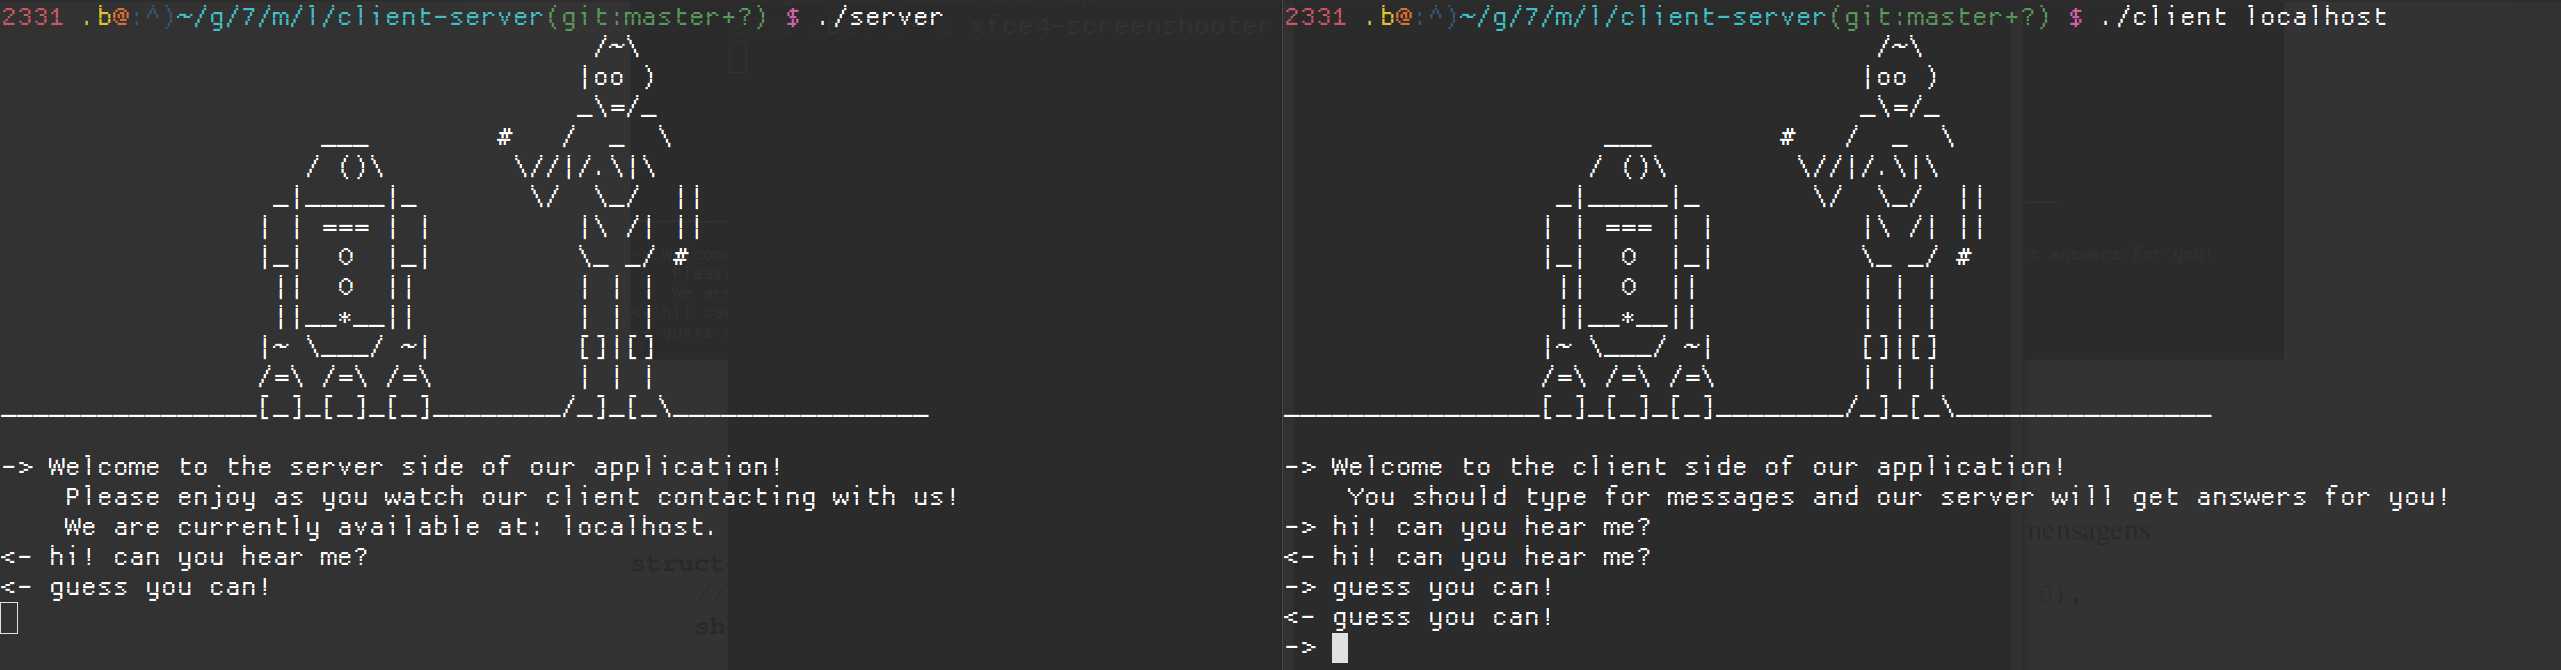
\includegraphics[width=0.45\textwidth]{img/sample.png}
    \caption{Exemplo de imagem}   
\end{center} 
\end{figure}

\section{server.c}
ablablabla aqui explica o servidor

\begin{lstlisting}[caption={aaaaaa}, label=Algorithm]
vou parar de code
\end{lstlisting}

e pretty much isso.

\section{Conclusões finais}

precisa mesmo?? coloquei mais por whatever.

%%% References %%%%%%%%%%%%%%%%%%%%%%%%%%%%%%%%%%%%%%%%%%%%%%%%%%%%%%%%%%%%%%%%%
%%
{\small
\bibliographystyle{unsrt}
\bibliography{refs}
}

\end{document}